%!TEX option = -enable-write18

\documentclass[9pt,svgnames,x11names]{beamer}

% counter for resuming enumerated list numbers
\newcounter{resumeenumi}
\newcommand{\suspend}{\setcounter{resumeenumi}{\theenumi}}
\newcommand{\resume}{\setcounter{enumi}{\theresumeenumi}}

\newcounter{saveenumi}
\newcommand{\seti}{\setcounter{saveenumi}{\value{enumi}}}
\newcommand{\conti}{\setcounter{enumi}{\value{saveenumi}}}
\resetcounteronoverlays{saveenumi}


% \newcounter{myexercisecounter}
% \newcommand{\suspendExerciseCounter}{\setcounter{myexercisecounter}{\theenumi}}
% \newcommand{\resumeExerciseCounter}{\setcounter{enumi}{\themyexercisecounter}}

\newcommand\lb{\linebreak}
\newcommand\pars{\par\smallskip}
\newcommand\parm{\par\medskip}
\newcommand\parb{\par\bigskip}

%left flushed minipage
\newcommand{\minit}[2][0.8]{
	\begin{minipage}[t]{#1\columnwidth}
		\raggedright
		#2
	\end{minipage}
}

%left flushed minipage
\newcommand{\mini}[2][0.8]{
	\begin{minipage}[c]{#1\columnwidth}
		\raggedright
		#2
	\end{minipage}
}

% centered minipage with text \raggedright
%\cmini[width]{content}
\newcommand{\cmini}[2][0.8]{
	\begin{center}
		\begin{minipage}{#1\columnwidth}
			\raggedright
			#2
		\end{minipage}
	\end{center}
}

\newcommand{\cfig}[2][1]{% centred, scaled graphic
	\begin{center}
		\includegraphics[scale=#1]{#2}
	\end{center}
}
% figure with tight border for photos
% \cfigb[saitMaroon]{borderwidth with unit}{scale}{image}
\newcommand{\cfigb}[4][structure]{
	% \usepackage{adjustbox}
	\setlength{\fboxrule}{1pt}
	\begin{center}
		\includegraphics[scale=#3, cframe= #1 #2]{#4}
	\end{center}
}
\newcommand{\imgbox}[3]{
	% \setlength{\fboxsep}{12pt}
	\includegraphics[scale=#1, cframe= structure #3]{#2}
}

% get x and y coordinates from a tikz coordinate
%\gettikzxy{A}{\ax}{\ay}
\makeatletter
\providecommand{\gettikzxy}[3]{%
	\tikz@scan@one@point\pgfutil@firstofone#1\relax
	\edef#2{\the\pgf@x}%
	\edef#3{\the\pgf@y}%
}
\makeatother

\definecolor{staticsRed}{RGB}{128, 30, 45}
\definecolor{mucus}{rgb}{0.55,0.53,0.31}
\definecolor{myGreen}{RGB}{0,150,0}
\definecolor{saitPurple}{RGB}{112,40,119}
\definecolor{saitDeepBlue}{RGB}{0, 99, 167}
\definecolor{saitBlue}{rgb}{0, 0.59, 0.85}

\definecolor{DarkKhakiMid}{RGB}{235, 228, 134}


%  \definecolor{saitRed}{RGB}{224,38,37} 

%  \definecolor{khaki}{RGB}{190, 183, 107}
%\definecolor{philpotBlue}{RGB}{13,69,120}
% \definecolor{dRed}{rgb}{0.7,0,0}
% \definecolor{blueGrey}{rgb}{0.4,0.48,0.53}
% \definecolor{white}{rgb}{1,1,1}
% \definecolor{dkgreen}{rgb}{0,0.5,0}
% \definecolor{greenyellow}{rgb}{0.9,0.9,0.5}
% \definecolor{flesh}{rgb}{1, 0.95, 0.8}
% \definecolor{wheat}{rgb}{.96, .87, .70}
% \definecolor{oldlace}{rgb}{.992, .96187, .902}
% \definecolor{snow}{rgb}{1, .98, .98}
% \definecolor{ghostwhite}{rgb}{.973, .973, 1}
% \definecolor{cornsilk}{rgb}{1, .973, .863}
% \definecolor{honeydew}{rgb}{.941, 1, .941}
% \definecolor{lavenderdark}{rgb}{.8, .8, .9529411}
% \definecolor{lavender}{rgb}{.902, .902, .980}
% \definecolor{lightblue}{rgb}{.8, .8, .95}
\definecolor{lightgray}{rgb}{.827, .827, .827}
% \definecolor{lightsteelblue}{rgb}{.690, .769, .871}
% \definecolor{lightturquoise}{rgb}{.686, .933, .933}
% \definecolor{darkgreen}{rgb}{.0, .392, .0}
% \definecolor{yellowgreen}{rgb}{.604, .804, .196}
% \definecolor{vlightblue}{rgb}{.88, .85, .95}
% \definecolor{khaki}{rgb}{.741, .718, .42}
% \definecolor{lightkhaki}{rgb}{1, .96, .7}
% \definecolor{almostwhite}{rgb}{1,.95,1}
% \definecolor{facegreen}{rgb}{.45, .5, .2}
% \definecolor{llllBlueGrey}{rgb}{0.8,0.96,1}
% \definecolor{lllBlueGrey}{rgb}{0.69,0.83,0.92}
% \definecolor{llBlueGrey}{rgb}{0.58,0.69,0.76}
% \definecolor{lBlueGrey}{rgb}{0.48,0.58,0.64}
% \definecolor{blueGrey}{rgb}{0.4,0.48,0.53}
% \definecolor{dBlueGrey}{rgb}{0.33,0.4,0.44}
% \definecolor{ddBlueGrey}{rgb}{0.28,0.33,0.37}
% \definecolor{dddBlueGrey}{rgb}{0.23,0.28,0.31}
% \definecolor{almostBlue}{rgb}{0.985,0.985,1}
% \definecolor{almostGreen}{rgb}{0.9,0.97,0.9}

% \definecolor{almostRed}{rgb}{0.95,0.875,0.8}
%  \definecolor{headerGrey}{RGB}{128,128,128}
%  \definecolor{headerGray}{RGB}{128,128,128}
% \definecolor{dHeaderGrey}{RGB}{96,96,96}
% \definecolor{ddHeaderGrey}{RGB}{64,64,64}
% \definecolor{dddHeaderGrey}{RGB}{32,32,32}
% \definecolor{lHeaderGrey}{RGB}{160,160,160}
% \definecolor{llHeaderGrey}{RGB}{192,192,192}
% \definecolor{lllHeaderGrey}{RGB}{224,224,224}
% \definecolor{philpotBlue}{RGB}{13,69,120}
% \definecolor{drabGreen}{RGB}{156,143,87}
% \definecolor{ground}{RGB}{153,153,51}
% \definecolor{gridLight}{rgb}{0.85,0.85,0.85}
% \definecolor{darkGreen}{rgb}{0,0.5,0}

% !TEX root = ../../statikz/statikz.tex

% % get x and y coordinates from a tikz coordinate, returned values in points
% \makeatletter
% \providecommand{\gettikzxy}[3]{%
%   \tikz@scan@one@point\pgfutil@firstofone#1\relax
%   \edef#2{\the\pgf@x}%
%   \edef#3{\the\pgf@y}%
% }
% \makeatother

%\Member{startpt}{endpt}{outer}{inner}{stroke}{height}{radius}{line width}
\providecommand{\Member}[8]{

  \def\topt{28.45274}
  \def\tocm{0.035146}
  % name the points
  \coordinate (start) at (#1); % coordinate
  \coordinate (end) at (#2); % coordinate
  
  \def\outer{#3} % color
  \def\inner{#4} % color
  \def\stroke{#5} % color
  \def\hi{#6} % cm
  \def\rad{#7} % cm
  \def\line{#8} % mm
  
  \gettikzxy{(start)}{\sx}{\sy}
  \gettikzxy{(end)}{\ex}{\ey}
  
  \coordinate(delta) at ($ (end)-(start) $);
  \gettikzxy{(delta)}{\dx}{\dy}
  
  \pgfmathparse{veclen(\dx, \dy)}% \pgfmathresult
  \let\length\pgfmathresult
  
  \pgfmathparse{\dx==0}%
  % \ifnum low-level TeX for integers
  \ifnum\pgfmathresult=1 % \dx == 0
    \pgfmathsetmacro{\rot}{\dy > 0 ? 90 : -90}
  \else
    \pgfmathsetmacro{\rot}{\dx > 0 ? atan(\dy / \dx) : 180 + atan(\dy / \dx)}
    
  \fi
  
  \fill[\inner] (#1) circle (.1mm); % node[black] {\sx, \sy};
  \fill[\inner] (#2) circle (.1mm); % node[black] {\ex, \ey};
  \begin{scope}	[rounded corners = 0.9*\rad cm, transform canvas = {rotate around = {\rot:(start)}}]
    \shadedraw[top color = \outer, bottom color = \outer, middle color = \inner, draw = \stroke, line width = \line mm] ($ (start)+(-0.5*\hi, 0.5*\hi) $) -- ++(\hi cm +\length pt, 0 ) -- ++(0, -\hi) -- ++ (-\hi cm -\length pt, 0) -- cycle;    
  \end{scope}
  
  % \draw[black] (start) circle (2mm);
  % \draw[black] (end) circle (2mm);
}


\newcommand{\PinnedConnection}[6][0]{
	\def\lrotate{#1}
	\def\lpin{#2}
	\def\lfill{#3}
	\def\ldraw{#4}
	\def\lscale{#5}
	\def\lwidth{#6}
	\def\h{1}
	\def\r{0.3}
	\begin{scope}[scale=\lscale, rotate=\lrotate]
		\filldraw[draw=\ldraw, fill=\lfill, line width=\lwidth mm] ($(\lpin) + (0.201*\h+1.0353*\r ,-0.75*\h)$) -- ++(105: 0.77646*\h+0.26795*\r) arc (15:165:\r) -- ++(-105:0.77646*\h+0.26795*\r) -- cycle;
		
		% \shadedraw[ball color=\lfill, draw=\ldraw, line width = \lwidth mm] (\lpin) circle (1.5mm);
		
		\filldraw[rounded corners=\lscale pt, draw=\ldraw, fill=\lfill, line width=\lwidth mm] ($ (\lpin) - (1,1) $) rectangle +(2,0.35);
	\end{scope}
}



%\Rone[rotate=0]{coordinate}{draw}{fill}{scale}{line width}
\newcommand{\RollerOne}[6][0]{
	\def\rotate{#1};
	\def\pin{#2}
	\def\lfill{#3}
	\def\ldraw{#4}
	\def\lscale{#5}
	\def\lwidth{#6}
	\def\h{1}
	\def\r{0.3}
	
	\begin{scope}[scale=\lscale, rotate=\rotate, line width=\lwidth mm]
		
		\shadedraw[ball color=\lfill!50, draw=\ldraw] ($ (\pin) + (0,-0.6*\h)$) circle (\h*4 mm);
		\filldraw[rounded corners=2pt, draw=\ldraw, fill=\lfill] ($(\pin) + (-0.52494*\h,-.8*\h)$) -- ++(1.05*\h, 0) -- ++(105:0.9059)arc(15:165:\r) -- cycle;
		\shadedraw[ball color=\lfill, draw=\ldraw] (\pin) circle (\lscale mm);
		\shadedraw[ball color=\lfill, draw=\ldraw] ($ (\pin) + (0,-0.6*\h)$) circle (\h*0.5 mm);
		
		
		
	\end{scope}
}



%\Roller[rotate=0]{coordinate}{draw}{fill}{scale}{line width}
\newcommand{\RollerThree}[6][0]{
	\def\rotate{#1};
	\def\pin{#2}
	\def\lfill{#3}
	\def\ldraw{#4}
	\def\lscale{#5};
	\def\lwidth{#6};
	\def\h{1}
	\def\r{0.3}
	\def\rr{0.15}
	\begin{scope}[scale=\lscale, rotate=\rotate, myshade/.style={outer color = \lfill!70!\ldraw, inner color=\lfill!25!white, draw=\ldraw!90!black, line width=\lwidth mm}]
		
		\shadedraw[myshade] ($(\pin) + (0,-\h+\rr)$) circle (\rr);
		\filldraw[\ldraw!50!black]($(\pin) + (0,-\h+\rr)$) circle (0.5mm);

		\shadedraw[myshade] ($(\pin) + (-0.325,-\h+\rr)$) circle (\rr);
		\filldraw[\ldraw!50!black]($(\pin) + (-0.325,-\h+\rr)$) circle (0.5mm);

		\shadedraw[myshade] ($(\pin) + (0.325,-\h+\rr)$) circle (\rr);
		\filldraw[\ldraw!50!black]($(\pin) + (0.325,-\h+\rr)$) circle (0.5mm);

		\filldraw[rounded corners= \lscale pt, draw=\ldraw, fill=\lfill, line width=\lwidth mm] ($(\pin) + (-0.52494*\h,-.8*\h)$) -- ++(1.05*\h, 0) -- ++(105:0.9059)arc(15:165:\r) -- cycle;

		\shadedraw[ball color=\lfill, \ldraw, line width=\lwidth mm] (\pin) circle (1.5mm);
		\filldraw[rounded corners=\lscale pt, draw=\ldraw, fill=\lfill, line width=\lwidth mm] ($ (\pin) - (0.55*\h,0.825*\h) $) rectangle +(1.1*\h,0.2*\h);
	\end{scope}
}




\providecommand{\RollerOnly}[6][0]{
	\def\rotate{#1};
	\def\pin{#2}
	\def\lfill{#3}
	\def\ldraw{#4}
	\def\lScale{#5};
	\def\lwidth{#6};
	\def\h{1}
	\def\r{0.3}
	\def\rr{0.2}
	\begin{scope}[scale=\lScale]
		\begin{scope}[roller/.style={outer color = \lfill, inner color=\lfill!30!black, draw=\ldraw!50!black, line width=\lwidth mm}]
			\shadedraw[roller] (\pin) circle (\h);
			\shadedraw[ball color=\lfill, line width=2*\lwidth pt] (\pin) circle (1.5mm);
		\end{scope}
	\end{scope}
}

\newcommand{\Rocker}[6][0]{
	\def\lrotate{#1};
	\def\lpin{#2}
	\def\lfill{#3}
	\def\ldraw{#4}
	\def\lscale{#5}
	\def\lwidth{#6}
	\def\h{1}
	\def\r{0.3}
	\begin{scope}[scale=\lscale, rotate=\lrotate]
        
        \filldraw[draw=\ldraw, fill=\lfill, line width = \lwidth mm] ($(\lpin) + (0,-\h)$)arc(-90:-57.54:\h) -- 
		++(105:0.95394)arc(15:165:\r) -- ++(-105:0.95394)arc(-122.458:-90:\h);

		\shadedraw[ball color=\lfill, draw=\ldraw, line width = \lwidth mm] (\lpin) circle (1.5mm);
		
	\end{scope}
}


\newcommand{\EyeConnection}[6][0]{
	\def\lrotate{#1};
	\def\lpin{#2}
	\def\lfill{#3}
	\def\ldraw{#4}
	\def\lscale{#5}
	\def\lwidth{#6}
	\def\h{1}
	\def\r{0.3}
	\begin{scope}[scale=\lscale, rotate=\lrotate]
		\filldraw[draw=\ldraw, fill=\lfill, line width=\lwidth mm] ($(\lpin) + (0.201*\h+1.0353*\r ,-0.75*\h)$) -- ++(105: 0.77646*\h+0.26795*\r) arc (15:165:\r) -- ++(-105:0.77646*\h+0.26795*\r) -- cycle;

		\fill[outer color=\lfill, inner color=black] (\lpin) circle (2.5mm);
		\filldraw[fill=white, draw=\ldraw, line width = \lwidth mm] (\lpin) circle (1.25mm);

		\filldraw[rounded corners=\lscale pt, draw=\ldraw, fill=\lfill, line width=\lwidth mm] ($ (\lpin) - (1,1) $) rectangle +(2,0.25);
	\end{scope}
}


\newcommand{\EyeConnectionB}[6][0]{
	\def\lrotate{#1};
	\def\lpin{#2}
	\def\lfill{#3}
	\def\ldraw{#4}
	\def\lscale{#5}
	\def\lwidth{#6}
	%\def\h{1.5}
	\def\r{0.3}
	\begin{scope}[scale=\lscale, rotate=\lrotate]
		\filldraw[draw=\ldraw, fill=\lfill, line width=\lwidth mm] ($(\lpin) + (-0.7,-1.25)$) arc(180:90:.2) -- ++(0.05,0)arc(-90:0:0.2) -- ++(0.05,0.65)arc(225:-45:0.28284)-- ++(0.05,-.65)arc(180:270:.2)-- ++(0.05,0)arc(90:0:0.2) -- cycle;
		\fill[outer color=\lfill, inner color=black, line width = 0] (\lpin) circle (2.25mm);
		\filldraw[fill=white, draw=\ldraw, line width = \lwidth mm] (\lpin) circle (1.25mm);

		\begin{scope}[even odd rule]
			\fill[\lfill] (\lpin) circle (2.5mm)
			(\lpin) circle (2.125mm);
		\end{scope}

		\filldraw[rounded corners=\lscale pt, draw=\ldraw, fill=\lfill, line width=\lwidth mm] ($ (\lpin) - (1,1.5) $) rectangle +(2,0.25);
	\end{scope}
}

% !TEX root = ../../statikz2020/statikz2020.tex

%\DLOne[rotate]{tl}{tr}{b}{fill}{draw}{spaces}{scale}{lineWidth}
\newcommand{\DLDown}[9][0]{
	\def\rotate{#1}
	\def\tl{#2}
	\def\tr{#3}
	\def\b{#4}
	\def\lfill{#5}
	\def\ldraw{#6}
	\def\spaces{#7}
	\def\lscale{#8}
	\def\llinewidth{#9}

	\def\tocm{0.0351459804}
	\providecommand\tiplength{5pt}

	\gettikzxy{(\tl)}{\tlx}{\tly};
	\gettikzxy{(\tr)}{\trx}{\try};
	\gettikzxy{(\b)}{\bx}{\by};

	\pgfmathparse{\trx-\tlx} \let\dx\pgfmathresult
	\pgfmathparse{\try-\tly} \let\dy\pgfmathresult
	\pgfmathparse{round(\tocm*\dx*100)/100} \let\dxcm\pgfmathresult
	\pgfmathparse{round(\tocm*\dy*100)/100} \let\dycm\pgfmathresult

	\coordinate (midBase) at (\tlx/2+\trx/2, \by);

	\gettikzxy{(midBase)}{\mx}{\my}
	\pgfmathparse{round(\tocm*\mx*100)/100} \let\mxcm\pgfmathresult
	\pgfmathparse{round(\tocm*\my*100)/100} \let\mycm\pgfmathresult


	\pgfmathparse{\dxcm/\spaces} \let\xspacing\pgfmathresult
	\pgfmathparse{\dycm/\spaces} \let\yspacing\pgfmathresult
	% \numarrows is actually one less than the number of arrows since we start a 0
	\pgfmathparse{\spaces-1} \let\numarrows\pgfmathresult

	\begin{scope}[scale=\lscale, rotate around ={\rotate:(midBase)}, line cap = round, line join = round, line width = \llinewidth mm]
		\fill[\lfill] (\tlx, \tly) -- (\trx, \try) -- (\trx, \by) -- (\tlx, \by);
		\draw[\ldraw, thin] (\tlx, \tly) -- (\trx, \try) -- (\trx, \by) -- (\tlx, \by) -- cycle;

		\pgfmathparse{abs(\try - \by)} \let\ryy\pgfmathresult
		\pgfmathparse{abs(\tly - \by)} \let\lyy\pgfmathresult

		% \pgfmathparse{\lyy>\tiplength && \ryy>\tiplength}
		% \ifnum\pgfmathresult=1
		% 	\draw[\ldraw, {Latex[length=\tiplength]}-{Latex[length=\tiplength]},line width=\llinewidth] (\tlx,\by) -- (\tlx, \tly) -- (\trx,\try) -- (\trx,\by);
		% \fi
		% \pgfmathparse{\lyy<\tiplength && \lyy>\tiplength/4 && \ryy>\tiplength}
		% \ifnum\pgfmathresult=1
		% 	\draw[\ldraw, {Latex[length=\lyy]}-{Latex[length=\tiplength]},line width=\llinewidth] (\tlx,\by) -- (\tlx, \tly) -- (\trx,\try) -- (\trx,\by);
		% \fi
		% \pgfmathparse{\lyy<=\tiplength/4 && \ryy>\tiplength}
		% \ifnum\pgfmathresult=1
		% 	\draw[\ldraw, -{Latex[length=\tiplength]},line width=\llinewidth] (\tlx,\by) -- (\tlx, \tly) -- (\trx,\try) -- (\trx,\by);
		% \fi
		% \pgfmathparse{\ryy<\tiplength && \ryy>\tiplength/4 && \lyy>\tiplength}
		% \ifnum\pgfmathresult=1
		% 	\draw[\ldraw, {Latex[length=\tiplength]}-{Latex[length=\ryy]},line width=\llinewidth] (\tlx,\by) -- (\tlx, \tly) -- (\trx,\try) -- (\trx,\by);
		% \fi
		% \pgfmathparse{\ryy<=\tiplength/4 && \lyy>\tiplength}
		% \ifnum\pgfmathresult=1
		% 	\draw[\ldraw, {Latex[length=\tiplength]}-,line width=\llinewidth] (\tlx,\by) -- (\tlx, \tly) -- (\trx,\try) -- (\trx,\by);
		% \fi
	
		\begin{scope}
			\clip (\tlx,\tly) -- (\trx, \try) -- (\trx,\by) -- (\tlx,\by) ;
			\foreach \i in {1,...,\numarrows}
			\def\x{\i*\xspacing}
			\def\y{\i*\yspacing}
			\draw[\ldraw, -{Latex[length=\tiplength]}, line width = \llinewidth pt] ($ (\tlx,\tly)+(\x,\y) $) -- ($ (\tlx,\by)+(\x,0) $);
		\end{scope}

		\pgfmathparse{\ryy>\tiplength}
		\ifnum\pgfmathresult=1
			\draw[\ldraw, -{Latex[length=\tiplength]},line width=\llinewidth] (\trx,\try) -- (\trx,\by);
		\fi

		\pgfmathparse{\lyy>\tiplength}
		\ifnum\pgfmathresult=1
			\draw[\ldraw, -{Latex[length=\tiplength]},line width=\llinewidth] (\tlx,\tly) -- (\tlx,\by);
		\fi

		
	\end{scope}
	
}

% !TEX root = ../../statikz2020/statikz2020.tex

%\DLOne[rotate]{tl}{tr}{b}{fill}{draw}{spaces}{scale}{lineWidth}
\newcommand{\DLUp}[9][0]{
	\def\rotate{#1}
	\def\tl{#2}
	\def\tr{#3}
	\def\b{#4}
	\def\lfill{#5}
	\def\ldraw{#6}
	\def\spaces{#7}
	\def\lscale{#8}
	\def\llinewidth{#9}
	
	\def\tocm{0.0351459804}
	\providecommand\tiplength{5pt}
	
	\gettikzxy{(\tl)}{\tlx}{\tly};
	\gettikzxy{(\tr)}{\trx}{\try};
	\gettikzxy{(\b)}{\bx}{\by};
	
	\pgfmathparse{\trx-\tlx} \let\dx\pgfmathresult
	\pgfmathparse{\try-\tly} \let\dy\pgfmathresult
	\pgfmathparse{round(\tocm*\dx*100)/100} \let\dxcm\pgfmathresult
	\pgfmathparse{round(\tocm*\dy*100)/100} \let\dycm\pgfmathresult
	
	\coordinate (midBase) at (\tlx/2+\trx/2, \by);
	
	\gettikzxy{(midBase)}{\mx}{\my}
	\pgfmathparse{round(\tocm*\mx*100)/100} \let\mxcm\pgfmathresult
	\pgfmathparse{round(\tocm*\my*100)/100} \let\mycm\pgfmathresult
	
	
	\pgfmathparse{\dxcm/\spaces} \let\xspacing\pgfmathresult
	\pgfmathparse{\dycm/\spaces} \let\yspacing\pgfmathresult
	% \numarrows is actually one less than the number of arrows since we start a 0
	\pgfmathparse{\spaces-1} \let\numarrows\pgfmathresult
	
	\begin{scope}[scale=\lscale, rotate around ={\rotate:(midBase)}, line cap = round, line join = round, line width = \llinewidth mm]
		\fill[\lfill] (\tlx, \tly) -- (\trx, \try) -- (\trx, \by) -- (\tlx, \by);
		\draw[\ldraw, thin] (\tlx, \tly) -- (\trx, \try) -- (\trx, \by) -- (\tlx, \by) -- cycle;
		
		\pgfmathparse{abs(\try - \by)} \let\ryy\pgfmathresult
		\pgfmathparse{abs(\tly - \by)} \let\lyy\pgfmathresult
		
		% \pgfmathparse{\lyy>\tiplength && \ryy>\tiplength}
		% \ifnum\pgfmathresult=1
		% 	\draw[\ldraw, {Latex[length=\tiplength]}-{Latex[length=\tiplength]},line width=\llinewidth] (\tlx,\by) -- (\tlx, \tly) -- (\trx,\try) -- (\trx,\by);
		% \fi
		% \pgfmathparse{\lyy<\tiplength && \lyy>\tiplength/4 && \ryy>\tiplength}
		% \ifnum\pgfmathresult=1
		% 	\draw[\ldraw, {Latex[length=\lyy]}-{Latex[length=\tiplength]},line width=\llinewidth] (\tlx,\by) -- (\tlx, \tly) -- (\trx,\try) -- (\trx,\by);
		% \fi
		% \pgfmathparse{\lyy<=\tiplength/4 && \ryy>\tiplength}
		% \ifnum\pgfmathresult=1
		% 	\draw[\ldraw, -{Latex[length=\tiplength]},line width=\llinewidth] (\tlx,\by) -- (\tlx, \tly) -- (\trx,\try) -- (\trx,\by);
		% \fi
		% \pgfmathparse{\ryy<\tiplength && \ryy>\tiplength/4 && \lyy>\tiplength}
		% \ifnum\pgfmathresult=1
		% 	\draw[\ldraw, {Latex[length=\tiplength]}-{Latex[length=\ryy]},line width=\llinewidth] (\tlx,\by) -- (\tlx, \tly) -- (\trx,\try) -- (\trx,\by);
		% \fi
		% \pgfmathparse{\ryy<=\tiplength/4 && \lyy>\tiplength}
		% \ifnum\pgfmathresult=1
		% 	\draw[\ldraw, {Latex[length=\tiplength]}-,line width=\llinewidth] (\tlx,\by) -- (\tlx, \tly) -- (\trx,\try) -- (\trx,\by);
		% \fi
		
		\begin{scope}
			\clip (\tlx,\tly) -- (\trx, \try) -- (\trx,\by) -- (\tlx,\by) ;
			\foreach \i in {1,...,\numarrows}
			\def\x{\i*\xspacing}
			\def\y{\i*\yspacing}
			\draw[\ldraw, {Latex[length=\tiplength]}-, line width = \llinewidth pt] ($ (\tlx,\tly)+(\x,\y) $) -- ($ (\tlx,\by)+(\x,0) $);
		\end{scope}
		
		\pgfmathparse{\ryy>\tiplength}
		\ifnum\pgfmathresult=1
			\draw[\ldraw, {Latex[length=\tiplength]}-,line width=\llinewidth] (\trx,\try) -- (\trx,\by);
		\fi
		
		\pgfmathparse{\lyy>\tiplength}
		\ifnum\pgfmathresult=1
			\draw[\ldraw, {Latex[length=\tiplength]}-,line width=\llinewidth] (\tlx,\tly) -- (\tlx,\by);
		\fi
		
		
	\end{scope}
	
}

\newcommand{\PenroseTri}[9][0]{
	\def\lrotate{#1};
	\def\lpin{#2}
	\def\len{#3}
	\def\ext{#4}
	\def\fillone{#5}
	\def\filltwo{#6}
	\def\fillthree{#7}
	\def\ddraw{#8}
	\def\lwidth{#9}
	
	% \coordinate (A) at (\lpin);
	% \coordinate (B) at ($(A)+(0:\len)$);
	% \coordinate (C) at ($(A)+(60:\len)$);	
	
	% \coordinate (AE) at ($(A)+(0:\ext)$);
	% \coordinate (AW) at ($(A)+(180:\ext)$);
	% \coordinate (ASW) at ($(A)+(240:\ext)$);
	% \coordinate (ANE) at ($(AE)+(60:\ext)$);
	
	% \coordinate (BE) at ($(B)+(0:\ext)$);
	% \coordinate (BNW) at ($(B)+(120:\ext)$);
	% \coordinate (BSE) at ($(B)+(-60:\ext)$);
	% \coordinate (BW) at ($(B)+(180:\ext)$);
	% \coordinate (BWNW) at ($(BNW)+(180:\ext)$);
	
	% \coordinate (CNE) at ($(C)+(60:\ext)$);
	% \coordinate (CNW) at ($(C)+(120:\ext)$);
	% \coordinate (CSW) at ($(C)+(240:\ext)$);
	% \coordinate (CS) at ($(CSW)+(-60:\ext)$);
	
	
	\begin{scope}[rotate around={\lrotate:(\lpin)}]
		% ugliness to avoid inadvertant use of common coordinate label clash from calling program
		\coordinate (aaaa) at (#2);
		\coordinate (bbbb) at ($(aaaa)+(0:\len)$);
		\coordinate (cccc) at ($(aaaa)+(60:\len)$);	
		
		\coordinate (aaaaE) at ($(aaaa)+(0:\ext)$);
		\coordinate (aaaaW) at ($(aaaa)+(180:\ext)$);
		\coordinate (aaaaSW) at ($(aaaa)+(240:\ext)$);
		\coordinate (aaaaNE) at ($(aaaaE)+(60:\ext)$);
		
		\coordinate (bbbbE) at ($(bbbb)+(0:\ext)$);
		\coordinate (bbbbNW) at ($(bbbb)+(120:\ext)$);
		\coordinate (bbbbSE) at ($(bbbb)+(-60:\ext)$);
		% \coordinate (BW) at ($(bbbb)+(180:\ext)$);
		\coordinate (bbbbWNW) at ($(bbbbNW)+(180:\ext)$);
		
		\coordinate (ccccNE) at ($(cccc)+(60:\ext)$);
		\coordinate (ccccNW) at ($(cccc)+(120:\ext)$);
		\coordinate (ccccSW) at ($(cccc)+(240:\ext)$);
		\coordinate (ccccS) at ($(ccccSW)+(-60:\ext)$);
		
		\shadedraw[draw=\ddraw, lower left = \filltwo!37!black, lower right=\filltwo, upper left=\filltwo, upper right=\filltwo, line width=\lwidth mm] (ccccNW)--(ccccNE)--(bbbbE)--(aaaaE)--(aaaaNE)--(bbbbNW)--cycle;
		
		\shadedraw[draw=\ddraw, upper left =\fillone!37!black, upper right = \fillone!25!black, lower left=\fillone, lower right =\fillone, line width=\lwidth mm] (ccccS)--(aaaaE)--(bbbbE)--(bbbbSE)--(aaaaSW)--(ccccSW)--cycle;
		
		\filldraw[draw=\ddraw, left color = \fillthree, right color=\fillthree!37!black, middle color=\fillthree, line width=\lwidth mm ] (ccccNW)--(bbbbNW)--(bbbbWNW)--(ccccSW)--(aaaaSW)--(aaaaW)--cycle;
		
		% % \shadedraw[ball color=\fillone, line width = \lwidth mm] (A) circle (0.75mm);
		% \shadedraw[ball color=\fillone, line width = \lwidth mm] (ANE) circle (0.5mm);
		% \shadedraw[ball color=\fillone, line width = \lwidth mm] (AE) circle (0.5mm);
		% \shadedraw[ball color=\fillone, line width = \lwidth mm] (AW) circle (0.5mm);
		% \shadedraw[ball color=\fillone, line width = \lwidth mm] (ASW) circle (0.5mm);
		
		% % \shadedraw[ball color=\filltwo, line width = \lwidth mm] (B) circle (0.75mm);
		% \shadedraw[ball color=\filltwo, line width = \lwidth mm] (BE) circle (0.5mm);
		% \shadedraw[ball color=\filltwo, line width = \lwidth mm] (BNW) circle (0.5mm);
		% \shadedraw[ball color=\filltwo, line width = \lwidth mm] (BSE) circle (0.5mm);
		% \shadedraw[ball color=\filltwo, line width = \lwidth mm] (BWNW) circle (0.5mm);
		
		% % \shadedraw[ball color=\fillthree, line width = \lwidth mm] (C) circle (0.75mm) ;
		% \shadedraw[ball color=\fillthree, line width = \lwidth mm] (CNE) circle (0.5mm);
		% \shadedraw[ball color=\fillthree, line width = \lwidth mm] (CNW) circle (0.5mm);
		% \shadedraw[ball color=\fillthree, line width = \lwidth mm] (CS) circle (0.5mm);
		% \shadedraw[ball color=\fillthree, line width = \lwidth mm] (CSW) circle (0.5mm);
		
		% \shadedraw[ball color=\fillone, line width = \lwidth mm] (C) circle (0.75mm);
		
	\end{scope}
}


\hypersetup{
    colorlinks,
    linkcolor=staticsRed, % table of contents
    urlcolor=staticsRed
}


\everymath{\displaystyle} 
\usefonttheme{professionalfonts}

\usepackage[absolute,overlay]{textpos}
\setlength{\TPHorizModule}{1.0cm}
\setlength{\TPVertModule}{\TPHorizModule}
\textblockorigin{0.0cm}{0.0cm}  %start all at upper left corner
\usepackage{bm}
\usepackage{verbatim} % for latex code in latex doc
\usepackage{tikz}
\usepackage{pgfmath}
\tikzset{every picture/.append style={line cap=round}}
\def\scale{1} % initialisation for pikz
\usetikzlibrary{calc} % only works within a path
% \usetikzlibrary{fpu}
\usetikzlibrary{math} % if then else etc.
\usetikzlibrary{arrows.meta}
\usetikzlibrary{shadings}
\usetikzlibrary{intersections}

\usetheme{Antibes}
\usecolortheme[named=staticsRed]{structure}
\setbeamertemplate{blocks}[rounded][shadow=false]
\setbeamertemplate{headline}{}%{\vspace{.1cm}}
\setbeamertemplate{navigation symbols}{} % empty braces suppresses all navigation symbols
\setbeamertemplate{footline}{
  \hfill
  \insertshorttitle
  \quad
  \insertsection
  \quad
  \insertsubsection
  \quad
  \insertframenumber/\inserttotalframenumber
  \quad{ }
  \vspace{0.125cm}
}
\addtobeamertemplate{footline}{\hypersetup{linkcolor=black}}{}
\setbeamertemplate{navigation symbols}{} % empty braces suppresses all navigation symbols
% \setbeamercolor{frametitle}{fg=white}
\setbeamertemplate{section in toc shaded}[default][50]
% \setbeamertemplate{subsection in toc}[subsections numbered]

\setcounter{tocdepth}{5}
% various hacks to get around (apparent?) Beamer titlepage constraints
\title[\color{black} Statikz\textcolor{staticsRed}{\;2018-\the\year}]{\Huge Statikz}
\subtitle{} % i.e., a blank line
\institute{\small Source code at: \lb{\footnotesize\url{https://github.com/dmorgorg/LaTeX2022}}}
\author{} % another blanky
\date{\small Last updated on \today}

%%%%%%%%%%%%%%%%%%%%%%%%%%%%%%%%%%%%%%%%%%%%%%%%%%%%%%%%%%%%%%%%%%%%%%%%%%%%%%%%%%%%%%%%%%%%%%%%%%%%%%%%
\begin{document}
%%%%%%%%%%%%%%%%%%%%%%%%%%%%%%%%%%%%%%%%%%%%%%%%%%%%%%%%%%%%%%%%%%%%%%%%%%%%%%%%%%%%%%%%%%%%%%%%%%%%%%%%

\begin{frame}[plain]
    \titlepage
\end{frame}

%%%%%%%%%%%%%%%%%%%%%%%%%%%%%%%%%%%%%%%%%%%%%%%%%%%%%%%%%%%%%%%%%%%%%%%%%%%%%%%%%%%%%%%%%%%%%%%%%%%%%%%%

\begin{frame}{Table of Contents}
    \begin{minipage}{0.9\textwidth}
        \tableofcontents
    \end{minipage}
    \vfill

\end{frame}
%%%%%%%%%%%%%%%%%%%%%%%%%%%%%%%%%%%%%%%%%%%%%%%%%%%%%%%%%%%%%%%%%%%%%%%%%%%%%%%%%%%%%%%%%%%%%%%%%%%%%%%%


%%%%%%%%%%%%%%%%%%%%%%%%%%%%%%%%%% Components %%%%%%%%%%%%%%%%%%%%%%%%%%%%%%%%%%%%%%%%%%%%%%%%%%%%%%%
\section{My Tikz Components}
%%%%%%%%%%%%%%%%%%%%%%%%%%%%%%%%%%%%%%%%%%%%%%%%%%%%%%%%%%%%%%%%%%%%%%%%%%%%%%%%%%%%%%%%%%%%%%%%%%%%

%%%%%%%%%%%%%%%%%%%%%%%%%%%%%%%%%%%%%%%%%%%%%%%%%%%%%%%%%%%%%%%%%%%%%%%%%%%%%%%%%%%%%%%%%%%%%%%%%%%%%%%%

% Note that use of verbatim within Beamer needs fragile setting for frame
% Also, verbatim environment cannot be inside curly braces, {\begin{verbatim}... blows up?

\begin{frame}[fragile]{Tikz Components :: Member}

    \small
    \begin{verbatim}
\Member{startpt}{endpt}{outer}{inner}{stroke}{height}{radius}{line width}
    \end{verbatim}
    \parb
    \vspace{2cm}
    \centering
    \resizebox{0.75\textwidth}{!}{%
        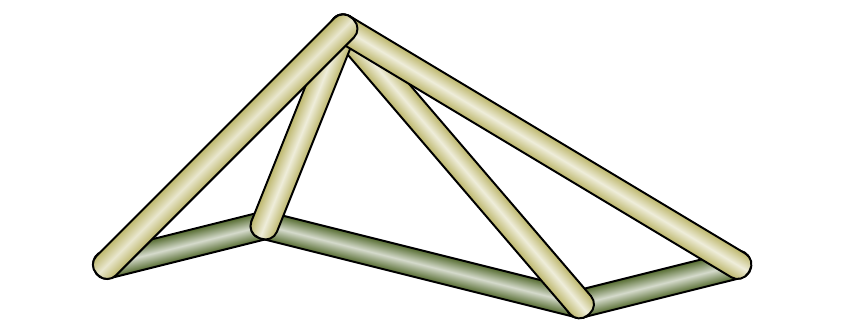
\begin{tikzpicture}
            \coordinate (A) at (0,0);
            \coordinate (B) at (3,3);
            \coordinate (C) at (8,0);
            \coordinate (D) at (6,-0.5);
            \coordinate (E) at (2,0.5);

            \Member{A}{E}{DarkOliveGreen}{DarkOliveGreen!25!white}{black}{0.35}{0.175}{.25}
            \Member{E}{D}{DarkOliveGreen}{DarkOliveGreen!25!white}{black}{0.35}{0.175}{.25}
            \Member{D}{C}{DarkOliveGreen}{DarkOliveGreen!25!white}{black}{0.35}{0.175}{.25}
            \Member{D}{B}{DarkKhaki}{DarkKhaki!25!white}{black}{0.35}{0.175}{.25}

            \Member{E}{B}{DarkKhaki}{DarkKhaki!25!white}{black}{0.35}{0.175}{.25}
            \Member{C}{B}{DarkKhaki}{DarkKhaki!25!white}{black}{0.35}{0.175}{.25}
            \Member{A}{B}{DarkKhaki}{DarkKhaki!33!white}{black}{0.35}{0.175}{.25}
            \fill[white] (-1,0) circle (0.1mm);
            \fill[white] (9,0) circle (0.1mm);
        \end{tikzpicture}
    }

\end{frame}
%%%%%%%%%%%%%%%%%%%%%%%%%%%%%%%%%%%%%%%%%%%%%%%%%%%%%%%%%%%%%%%%%%%%%%%%%%%%%%%%%%%%%%%%%%%%%%%%%%%%

\begin{frame}[fragile]{Tikz Components :: Some Example Member Colors}

    \def\horiz{4}
    \def\vert{-0.55}
    \small


    \centering
    \resizebox{0.95\textwidth}{!}{%
        \begin{tikzpicture}
            \coordinate (A) at (0,0);
            \coordinate (AA) at ($(A)+(5,0)$);
            \coordinate (AAA) at ($(AA)+(\horiz,0)$);

            \coordinate (B) at ($(A)+(0,\vert)$);
            \coordinate (BB) at ($(B)+(5,0)$);
            \coordinate (BBB) at ($(BB)+(\horiz,0)$);

            \coordinate (C) at ($(B)+(0,\vert)$);
            \coordinate (CC) at ($(C)+(5,0)$);
            \coordinate (CCC) at ($(CC)+(\horiz,0)$);

            \coordinate (D) at ($(C)+(0,\vert)$);
            \coordinate (DD) at ($(D)+(5,0)$);
            \coordinate (DDD) at ($(DD)+(\horiz,0)$);

            \coordinate (E) at ($(D)+(0,\vert)$);
            \coordinate (EE) at ($(E)+(5,0)$);
            \coordinate (EEE) at ($(EE)+(\horiz,0)$);

            \coordinate (F) at ($(E)+(0,\vert)$);
            \coordinate (FF) at ($(F)+(5,0)$);
            \coordinate (FFF) at ($(FF)+(\horiz,0)$);

            \coordinate (G) at ($(F)+(0,\vert)$);
            \coordinate (GG) at ($(G)+(5,0)$);
            \coordinate (GGG) at ($(GG)+(\horiz,0)$);

            \coordinate (H) at ($(G)+(0,\vert)$);
            \coordinate (HH) at ($(H)+(5,0)$);
            \coordinate (HHH) at ($(HH)+(\horiz,0)$);

            \coordinate (I) at ($(H)+(0,-1)$);
            \coordinate (II) at ($(I)+(5,0)$);
            \coordinate (III) at ($(II)+(\horiz,0)$);

            \coordinate (J) at ($(I)+(0,\vert)$);
            \coordinate (JJ) at ($(J)+(5,0)$);
            \coordinate (JJJ) at ($(JJ)+(\horiz,0)$);

            \coordinate (K) at ($(J)+(0,\vert)$);
            \coordinate (KK) at ($(K)+(5,0)$);
            \coordinate (KKK) at ($(KK)+(\horiz,0)$);

            \coordinate (L) at ($(K)+(0,\vert)$);
            \coordinate (LL) at ($(L)+(5,0)$);
            \coordinate (LLL) at ($(LL)+(\horiz,0)$);

            \coordinate (M) at ($(L)+(0,\vert)$);
            \coordinate (MM) at ($(M)+(5,0)$);
            \coordinate (MMM) at ($(MM)+(\horiz,0)$);

            \coordinate (N) at ($(M)+(0,\vert)$);
            \coordinate (NN) at ($(N)+(5,0)$);
            \coordinate (NNN) at ($(NN)+(\horiz,0)$);

            \coordinate (O) at ($(N)+(0,\vert)$);
            \coordinate (OO) at ($(O)+(5,0)$);
            \coordinate (OOO) at ($(OO)+(\horiz,0)$);

            \Member{A}{AA}{DarkKhaki}{DarkKhaki!25!white}{black}{0.35}{0.175}{.125}
            \shadedraw[ball color=DarkKhaki] (A) circle (1mm);
            \shadedraw[ball color=DarkKhaki] (AA) circle (1mm);
            \draw[thin, DarkKhaki] ($(AA)+(0.5,0)$)--(AAA);
            \node[fill=white, inner sep=0.25cm] at (AAA) {\textcolor{DarkKhaki}{\{DarkKhaki\}\{DarkKhaki!25!white\}}};

            \Member{B}{BB}{DarkOliveGreen}{DarkOliveGreen!25!white}{black}{0.35}{0.175}{.125}
            \shadedraw[ball color=DarkOliveGreen] (B) circle (1mm);
            \shadedraw[ball color=DarkOliveGreen] (BB) circle (1mm);
            \draw[thin, DarkOliveGreen] ($(BB)+(0.5,0)$)--(BBB);
            \node[fill=white, inner sep=0.25cm] at (BBB) {\textcolor{DarkOliveGreen}{\{DarkOliveGreen\}\{DarkOliveGreen!25!white\}}};

            \Member{C}{CC}{DarkGoldenrod}{DarkGoldenrod!22!white}{black}{0.35}{0.175}{.125}
            \shadedraw[ball color=DarkGoldenrod] (C) circle (1mm);
            \shadedraw[ball color=DarkGoldenrod] (CC) circle (1mm);
            \draw[thin, DarkGoldenrod] ($(CC)+(0.5,0)$)--(CCC);
            \node[fill=white, inner sep=0.25cm] at (CCC) {\textcolor{DarkGoldenrod}{\{DarkGoldenrod\}\{DarkGoldenrod!25!white\}}};

            \Member{D}{DD}{Olive}{Olive!25!white}{black}{0.35}{0.175}{.125}
            \shadedraw[ball color=Olive] (D) circle (1mm);
            \shadedraw[ball color=Olive] (DD) circle (1mm);
            \draw[thin, Olive] ($(DD)+(0.5,0)$)--(DDD);
            \node[fill=white, inner sep=0.25cm] at (DDD) {\textcolor{Olive}{\{Olive\}\{Olive!25!white\}}};

            \Member{E}{EE}{OliveDrab}{OliveDrab!25!white}{black}{0.35}{0.175}{.125}
            \shadedraw[ball color=OliveDrab] (E) circle (1mm);
            \shadedraw[ball color=OliveDrab] (EE) circle (1mm);
            \draw[thin, OliveDrab] ($(EE)+(0.5,0)$)--(EEE);
            \node[fill=white, inner sep=0.25cm] at (EEE) {\textcolor{OliveDrab}{\{OliveDrab\}\{OliveDrab!25!white\}}};

            \Member{F}{FF}{Sienna}{Sienna!25!white}{black}{0.35}{0.175}{.125}
            \shadedraw[ball color=Sienna] (F) circle (1mm);
            \shadedraw[ball color=Sienna] (FF) circle (1mm);
            \draw[thin, Sienna] ($(FF)+(0.5,0)$)--(FFF);
            \node[fill=white, inner sep=0.25cm] at (FFF) {\textcolor{Sienna}{\{Sienna\}\{Sienna!25!white\}}};

            \Member{G}{GG}{BurlyWood}{BurlyWood!25!white}{black}{0.35}{0.175}{.125}
            \shadedraw[ball color=BurlyWood] (G) circle (1mm);
            \shadedraw[ball color=BurlyWood] (GG) circle (1mm);
            \draw[thin, BurlyWood] ($(GG)+(0.5,0)$)--(GGG);
            \node[fill=white, inner sep=0.25cm] at (GGG) {\textcolor{BurlyWood}{\{BurlyWood\}\{BurlyWood!25!white\}}};

            \Member{H}{HH}{Tan}{Tan!25!white}{black}{0.35}{0.175}{.125}
            \shadedraw[ball color=Tan] (H) circle (1mm);
            \shadedraw[ball color=Tan] (HH) circle (1mm);
            \draw[thin, Tan] ($(HH)+(0.5,0)$)--(HHH);
            \node[fill=white, inner sep=0.25cm] at (HHH) {\textcolor{Tan}{\{Tan\}\{Tan!25!white\}}};

            \Member{I}{II}{PeachPuff4}{PeachPuff2}{black}{0.35}{0.175}{.125}
            \shadedraw[ball color=PeachPuff4] (I) circle (1mm);
            \shadedraw[ball color=PeachPuff4] (II) circle (1mm);
            \draw[thin, PeachPuff4] ($(II)+(0.5,0)$)--(III);
            \node[fill=white, inner sep=0.25cm] at (III) {\textcolor{PeachPuff4}{\{PeachPuff4\}\{PeachPuff2\}}};

            \Member{J}{JJ}{Bisque4}{Bisque2}{black}{0.35}{0.175}{.125}
            \shadedraw[ball color=Bisque4] (J) circle (1mm);
            \shadedraw[ball color=Bisque4] (JJ) circle (1mm);
            \draw[thin, Bisque4] ($(JJ)+(0.5,0)$)--(JJJ);
            \node[fill=white, inner sep=0.25cm] at (JJJ) {\textcolor{Bisque4}{\{Bisque4\}\{Bisque2\}}};

            \Member{K}{KK}{Burlywood4}{Burlywood2}{black}{0.35}{0.175}{.125}
            \shadedraw[ball color=Burlywood4] (K) circle (1mm);
            \shadedraw[ball color=Burlywood4] (KK) circle (1mm);
            \draw[thin, Burlywood4] ($(KK)+(0.5,0)$)--(KKK);
            \node[fill=white, inner sep=0.25cm] at (KKK) {\textcolor{Burlywood4}{\{Burlywood4\}\{Burlywood2\}}};

            \Member{L}{LL}{Cornsilk4}{Cornsilk2}{black}{0.35}{0.175}{.125}
            \shadedraw[ball color=Cornsilk4] (L) circle (1mm);
            \shadedraw[ball color=Cornsilk4] (LL) circle (1mm);
            \draw[thin, Cornsilk4] ($(LL)+(0.5,0)$)--(LLL);
            \node[fill=white, inner sep=0.25cm] at (LLL) {\textcolor{Cornsilk4}{\{Cornsilk4\}\{Cornsilk2\}}};

            \Member{M}{MM}{Honeydew4}{Honeydew2}{black}{0.35}{0.175}{.125}
            \shadedraw[ball color=Honeydew4] (M) circle (1mm);
            \shadedraw[ball color=Honeydew4] (MM) circle (1mm);
            \draw[thin, Honeydew4] ($(MM)+(0.5,0)$)--(MMM);
            \node[fill=white, inner sep=0.25cm] at (MMM) {\textcolor{Honeydew4}{\{Honeydew4\}\{Honeydew2\}}};

            \Member{N}{NN}{Seashell4}{Seashell2}{black}{0.35}{0.175}{.125}
            \shadedraw[ball color=Seashell4] (N) circle (1mm);
            \shadedraw[ball color=Seashell4] (NN) circle (1mm);
            \draw[thin, Seashell4] ($(NN)+(0.5,0)$)--(NNN);
            \node[fill=white, inner sep=0.25cm] at (NNN) {\textcolor{Seashell4}{\{Seashell4\}\{Seashell2\}}};

            \Member{O}{OO}{Wheat4}{Wheat2}{black}{0.35}{0.175}{.125}
            \shadedraw[ball color=Wheat4] (O) circle (1mm);
            \shadedraw[ball color=Wheat4] (OO) circle (1mm);
            \draw[thin, Wheat4] ($(OO)+(0.5,0)$)--(OOO);
            \node[fill=white, inner sep=0.25cm] at (OOO) {\textcolor{Wheat4}{\{Wheat4\}\{Wheat2\}}};
        \end{tikzpicture}
    }

\end{frame}
%%%%%%%%%%%%%%%%%%%%%%%%%%%%%%%%%%%%%%%%%%%%%%%%%%%%%%%%%%%%%%%%%%%%%%%%%%%%%%%%%%%%%%%%%%%%%%%%%%%%

\begin{frame}[fragile]{Tikz Components :: Some More Member Colors}
    \small

    \parb
    \centering
    \resizebox{0.75\textwidth}{!}{%
        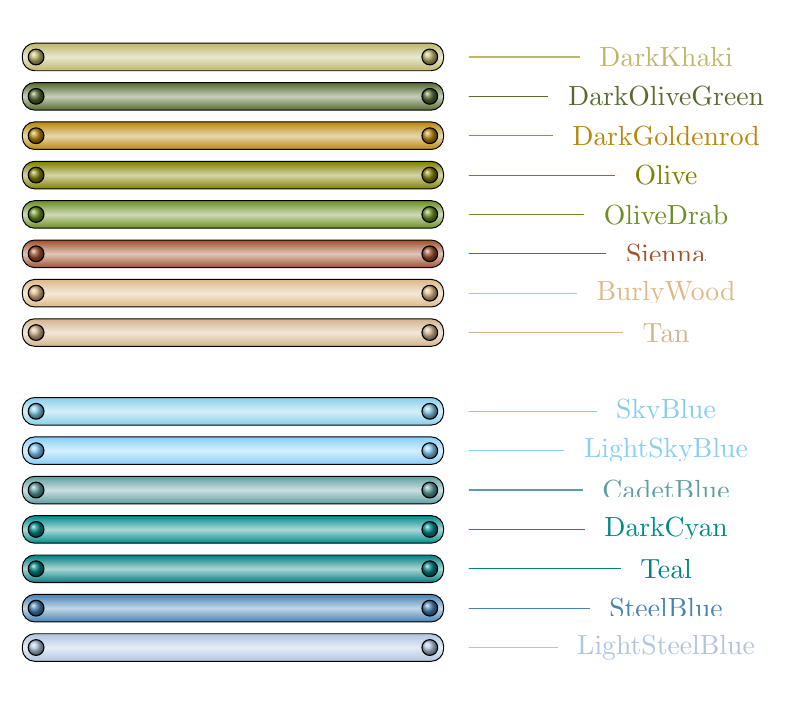
\begin{tikzpicture}
            \coordinate (A) at (0,0);
            \coordinate (AA) at ($(A)+(5,0)$);
            \coordinate (AAA) at ($(AA)+(3,0)$);

            \coordinate (B) at ($(A)+(0,-0.5)$);
            \coordinate (BB) at ($(B)+(5,0)$);
            \coordinate (BBB) at ($(BB)+(3,0)$);

            \coordinate (C) at ($(B)+(0,-0.5)$);
            \coordinate (CC) at ($(C)+(5,0)$);
            \coordinate (CCC) at ($(CC)+(3,0)$);

            \coordinate (D) at ($(C)+(0,-0.5)$);
            \coordinate (DD) at ($(D)+(5,0)$);
            \coordinate (DDD) at ($(DD)+(3,0)$);

            \coordinate (E) at ($(D)+(0,-0.5)$);
            \coordinate (EE) at ($(E)+(5,0)$);
            \coordinate (EEE) at ($(EE)+(3,0)$);

            \coordinate (F) at ($(E)+(0,-0.5)$);
            \coordinate (FF) at ($(F)+(5,0)$);
            \coordinate (FFF) at ($(FF)+(3,0)$);

            \coordinate (G) at ($(F)+(0,-0.5)$);
            \coordinate (GG) at ($(G)+(5,0)$);
            \coordinate (GGG) at ($(GG)+(3,0)$);

            \coordinate (H) at ($(G)+(0,-0.5)$);
            \coordinate (HH) at ($(H)+(5,0)$);
            \coordinate (HHH) at ($(HH)+(3,0)$);

            \coordinate (I) at ($(H)+(0,-1)$);
            \coordinate (II) at ($(I)+(5,0)$);
            \coordinate (III) at ($(II)+(3,0)$);

            \coordinate (J) at ($(I)+(0,-0.5)$);
            \coordinate (JJ) at ($(J)+(5,0)$);
            \coordinate (JJJ) at ($(JJ)+(3,0)$);

            \coordinate (K) at ($(J)+(0,-0.5)$);
            \coordinate (KK) at ($(K)+(5,0)$);
            \coordinate (KKK) at ($(KK)+(3,0)$);

            \coordinate (L) at ($(K)+(0,-0.5)$);
            \coordinate (LL) at ($(L)+(5,0)$);
            \coordinate (LLL) at ($(LL)+(3,0)$);

            \coordinate (M) at ($(L)+(0,-0.5)$);
            \coordinate (MM) at ($(M)+(5,0)$);
            \coordinate (MMM) at ($(MM)+(3,0)$);

            \coordinate (N) at ($(M)+(0,-0.5)$);
            \coordinate (NN) at ($(N)+(5,0)$);
            \coordinate (NNN) at ($(NN)+(3,0)$);

            \coordinate (O) at ($(N)+(0,-0.5)$);
            \coordinate (OO) at ($(O)+(5,0)$);
            \coordinate (OOO) at ($(OO)+(3,0)$);

            \Member{A}{AA}{DarkKhaki}{DarkKhaki!33!white}{black}{0.35}{0.175}{.125}
            \shadedraw[ball color=DarkKhaki] (A) circle (1mm);
            \shadedraw[ball color=DarkKhaki] (AA) circle (1mm);
            \draw[thin, DarkKhaki] ($(AA)+(0.5,0)$)--(AAA);
            \node[fill=white, inner sep=0.25cm] at (AAA) {\textcolor{DarkKhaki}{DarkKhaki}};

            \Member{B}{BB}{DarkOliveGreen}{DarkOliveGreen!33!white}{black}{0.35}{0.175}{.125}
            \shadedraw[ball color=DarkOliveGreen] (B) circle (1mm);
            \shadedraw[ball color=DarkOliveGreen] (BB) circle (1mm);
            \draw[thin, DarkOliveGreen] ($(BB)+(0.5,0)$)--(BBB);
            \node[fill=white, inner sep=0.25cm] at (BBB) {\textcolor{DarkOliveGreen}{DarkOliveGreen}};

            \Member{C}{CC}{DarkGoldenrod}{DarkGoldenrod!33!white}{black}{0.35}{0.175}{.125}
            \shadedraw[ball color=DarkGoldenrod] (C) circle (1mm);
            \shadedraw[ball color=DarkGoldenrod] (CC) circle (1mm);
            \draw[thin, DarkGoldenrod] ($(CC)+(0.5,0)$)--(CCC);
            \node[fill=white, inner sep=0.25cm] at (CCC) {\textcolor{DarkGoldenrod}{DarkGoldenrod}};

            \Member{D}{DD}{Olive}{Olive!33!white}{black}{0.35}{0.175}{.125}
            \shadedraw[ball color=Olive] (D) circle (1mm);
            \shadedraw[ball color=Olive] (DD) circle (1mm);
            \draw[thin, Olive] ($(DD)+(0.5,0)$)--(DDD);
            \node[fill=white, inner sep=0.25cm] at (DDD) {\textcolor{Olive}{Olive}};

            \Member{E}{EE}{OliveDrab}{OliveDrab!33!white}{black}{0.35}{0.175}{.125}
            \shadedraw[ball color=OliveDrab] (E) circle (1mm);
            \shadedraw[ball color=OliveDrab] (EE) circle (1mm);
            \draw[thin, OliveDrab] ($(EE)+(0.5,0)$)--(EEE);
            \node[fill=white, inner sep=0.25cm] at (EEE) {\textcolor{OliveDrab}{OliveDrab}};

            \Member{F}{FF}{Sienna}{Sienna!33!white}{black}{0.35}{0.175}{.125}
            \shadedraw[ball color=Sienna] (F) circle (1mm);
            \shadedraw[ball color=Sienna] (FF) circle (1mm);
            \draw[thin, Sienna] ($(FF)+(0.5,0)$)--(FFF);
            \node[fill=white, inner sep=0.25cm] at (FFF) {\textcolor{Sienna}{Sienna}};

            \Member{G}{GG}{BurlyWood}{BurlyWood!33!white}{black}{0.35}{0.175}{.125}
            \shadedraw[ball color=BurlyWood] (G) circle (1mm);
            \shadedraw[ball color=BurlyWood] (GG) circle (1mm);
            \draw[thin, BurlyWood] ($(GG)+(0.5,0)$)--(GGG);
            \node[fill=white, inner sep=0.25cm] at (GGG) {\textcolor{BurlyWood}{BurlyWood}};

            \Member{H}{HH}{Tan}{Tan!33!white}{black}{0.35}{0.175}{.125}
            \shadedraw[ball color=Tan] (H) circle (1mm);
            \shadedraw[ball color=Tan] (HH) circle (1mm);
            \draw[thin, Tan] ($(HH)+(0.5,0)$)--(HHH);
            \node[fill=white, inner sep=0.25cm] at (HHH) {\textcolor{Tan}{Tan}};

            \Member{I}{II}{SkyBlue}{SkyBlue!33!white}{black}{0.35}{0.175}{.125}
            \shadedraw[ball color=SkyBlue] (I) circle (1mm);
            \shadedraw[ball color=SkyBlue] (II) circle (1mm);
            \draw[thin, SkyBlue] ($(II)+(0.5,0)$)--(III);
            \node[fill=white, inner sep=0.25cm] at (III) {\textcolor{SkyBlue}{SkyBlue}};

            \Member{J}{JJ}{LightSkyBlue}{LightSkyBlue!33!white}{black}{0.35}{0.175}{.125}
            \shadedraw[ball color=LightSkyBlue] (J) circle (1mm);
            \shadedraw[ball color=LightSkyBlue] (JJ) circle (1mm);
            \draw[thin, LightSkyBlue] ($(JJ)+(0.5,0)$)--(JJJ);
            \node[fill=white, inner sep=0.25cm] at (JJJ) {\textcolor{LightSkyBlue}{LightSkyBlue}};

            \Member{K}{KK}{CadetBlue}{CadetBlue!33!white}{black}{0.35}{0.175}{.125}
            \shadedraw[ball color=CadetBlue] (K) circle (1mm);
            \shadedraw[ball color=CadetBlue] (KK) circle (1mm);
            \draw[thin, CadetBlue] ($(KK)+(0.5,0)$)--(KKK);
            \node[fill=white, inner sep=0.25cm] at (KKK) {\textcolor{CadetBlue}{CadetBlue}};

            \Member{L}{LL}{DarkCyan}{DarkCyan!33!white}{black}{0.35}{0.175}{.125}
            \shadedraw[ball color=DarkCyan] (L) circle (1mm);
            \shadedraw[ball color=DarkCyan] (LL) circle (1mm);
            \draw[thin, DarkCyan] ($(LL)+(0.5,0)$)--(LLL);
            \node[fill=white, inner sep=0.25cm] at (LLL) {\textcolor{DarkCyan}{DarkCyan}};

            \Member{M}{MM}{Teal}{Teal!33!white}{black}{0.35}{0.175}{.125}
            \shadedraw[ball color=Teal] (M) circle (1mm);
            \shadedraw[ball color=Teal] (MM) circle (1mm);
            \draw[thin, Teal] ($(MM)+(0.5,0)$)--(MMM);
            \node[fill=white, inner sep=0.25cm] at (MMM) {\textcolor{Teal}{Teal}};

            \Member{N}{NN}{SteelBlue}{SteelBlue!33!white}{black}{0.35}{0.175}{.125}
            \shadedraw[ball color=SteelBlue] (N) circle (1mm);
            \shadedraw[ball color=SteelBlue] (NN) circle (1mm);
            \draw[thin, SteelBlue] ($(NN)+(0.5,0)$)--(NNN);
            \node[fill=white, inner sep=0.25cm] at (NNN) {\textcolor{SteelBlue}{SteelBlue}};

            \Member{O}{OO}{LightSteelBlue}{LightSteelBlue!33!white}{black}{0.35}{0.175}{.125}
            \shadedraw[ball color=LightSteelBlue] (O) circle (1mm);
            \shadedraw[ball color=LightSteelBlue] (OO) circle (1mm);
            \draw[thin, LightSteelBlue] ($(OO)+(0.5,0)$)--(OOO);
            \node[fill=white, inner sep=0.25cm] at (OOO) {\textcolor{LightSteelBlue}{LightSteelBlue}};
        \end{tikzpicture}
    }

\end{frame}

%%%%%%%%%%%%%%%%%%%%%%%%%%%%%%%%%%%%%%%%%%%%%%%%%%%%%%%%%%%%%%%%%%%%%%%%%%%%%%%%%%%%%%%%%%%%%%%%%%%

\begin{frame}[fragile]{Tikz Components :: PinnedConnection}

    \small
    \begin{verbatim}
\PinnedConnection[rotate=0]{coordinate}{fill}{draw}{scale}{line width}
   
    \end{verbatim}

    \centering
    \vspace{1cm}

    \tikz{
        \coordinate (A) at (0,0);
        % \PinnedConnection[rotate=0]{coordinate}{fill}{draw}{scale}{line width}
        \PinnedConnection{A}{DarkKhaki}{Black}{1}{0.25}
    }

\end{frame}

%%%%%%%%%%%%%%%%%%%%%%%%%%%%%%%%%%%%%%%%%%%%%%%%%%%%%%%%%%%%%%%%%%%%%%%%%%%%%%%%%%%%%%%%%%%%%%%%%%%

\begin{frame}[fragile]{Tikz Components :: RollerOne}

    \footnotesize
    \begin{verbatim}
    \RollerOne[rotate=0]{coordinate}{fill}{draw}{scale}{line width}
  \end{verbatim}

    \centering
    \vspace{1cm}

    \tikz{
        \coordinate (A) at (0,0);
        \RollerOne{A}{DarkKhaki}{Black}{1}{0.25}
    }

\end{frame}

%%%%%%%%%%%%%%%%%%%%%%%%%%%%%%%%%%%%%%%%%%%%%%%%%%%%%%%%%%%%%%%%%%%%%%%%%%%%%%%%%%%%%%%%%%%%%%%%%%%

\begin{frame}[fragile]{Tikz Components :: RollerThree}

    \footnotesize
    \begin{verbatim}
    \RollerThree[rotate=0]{coordinate}{fill}{draw}{scale}{line width}
  \end{verbatim}

    \vspace{1cm}
    \centering

    \tikz{
        \coordinate (A) at (0,0);
        \RollerThree{A}{DarkKhaki}{Black}{1}{0.25}
    }

\end{frame}

%%%%%%%%%%%%%%%%%%%%%%%%%%%%%%%%%%%%%%%%%%%%%%%%%%%%%%%%%%%%%%%%%%%%%%%%%%%%%%%%%%%%%%%%%%%%%%%%%%%

\begin{frame}[fragile]{Tikz Components :: RollerOnly}

    \footnotesize
    \begin{verbatim}
    \RollerOnly[rotate=0]{coordinate}{fill}{draw}{scale}{line width}
  \end{verbatim}

    \centering
    \vspace{1cm}

    \tikz{
        \coordinate (A) at (0,0);
        \RollerOnly{A}{DarkKhaki}{Black}{1}{0.25}
    }

\end{frame}

%%%%%%%%%%%%%%%%%%%%%%%%%%%%%%%%%%%%%%%%%%%%%%%%%%%%%%%%%%%%%%%%%%%%%%%%%%%%%%%%%%%%%%%%%%%%%%%%%%

\begin{frame}[fragile]{Tikz Components :: Rocker}

    \footnotesize
    \begin{verbatim}
    \Rocker[rotate=0]{coordinate}{fill}{draw}{scale}{line width}
  \end{verbatim}
    \centering
    \vspace{1cm}

    \tikz{
        \coordinate (A) at (0,0);
        % \Rocker[rotate=0]{coordinate}{fill}{draw}{scale}{line width}
        \Rocker{A}{DarkKhaki}{Black}{1}{0.25}
    }

\end{frame}

%%%%%%%%%%%%%%%%%%%%%%%%%%%%%%%%%%%%%%%%%%%%%%%%%%%%%%%%%%%%%%%%%%%%%%%%%%%%%%%%%%%%%%%%%%%%%%%%%%%

\begin{frame}[fragile]{Tikz Components :: EyeConnection}

    \footnotesize
    \begin{verbatim}
    \EyeConnection[rotate=0]{coordinate}{fill}{draw}{scale}{line width}
  \end{verbatim}

    \vspace{1cm}
    \centering

    \tikz{
        \coordinate (A) at (0,0);
        \EyeConnection{A}{DarkKhaki}{Black}{1}{0.25}
    }

\end{frame}

%%%%%%%%%%%%%%%%%%%%%%%%%%%%%%%%%%%%%%%%%%%%%%%%%%%%%%%%%%%%%%%%%%%%%%%%%%%%%%%%%%%%%%%%%%%%%%%%%%

\begin{frame}[fragile]{Tikz Components :: EyeConnectionB}

    \small
    \begin{verbatim}
    \EyeConnectionB[rotate=0]{coordinate}{fill}{draw}{scale}{line width}
  \end{verbatim}

    \vspace{1cm}
    \centering
    \tikz{
        \coordinate (A) at (0,0);
        \coordinate (B) at (0,-1);
        \EyeConnectionB{A}{DarkKhaki}{Black}{1}{0.25}
    }

\end{frame}

%%%%%%%%%%%%%%%%%%%%%%%%%%%%%%%%%%%%%%%%%%%%%%%%%%%%%%%%%%%%%%%%%%%%%%%%%%%%%%%%%%%%%%%%%%%%%%%%%%

\begin{frame}[fragile]{Tikz Components :: DLDown}

    \footnotesize
    \begin{verbatim}
    \DLDown[rotate]{tl}{tr}{b}{fill}{draw}{spaces}{scale}{lineWidth}

    \DLDown[25]{A}{B}{C}{SlateGray3}{SlateGray4!75!black}{5}{1}{0.375}
  \end{verbatim}
    \centering
    \tikz{
        \coordinate (A) at (0,0);
        \coordinate (B) at (4,3);
        \coordinate (C) at (0,-1);
        % \DLDown[rotate]{tl}{tr}{b}{fill}{draw}{spaces}{scale}{lineWidth}
        \DLDown[25]{A}{B}{C}{SlateGray3}{SlateGray4!75!black}{5}{1}{0.375}
    }

\end{frame}

%%%%%%%%%%%%%%%%%%%%%%%%%%%%%%%%%%%%%%%%%%%%%%%%%%%%%%%%%%%%%%%%%%%%%%%%%%%%%%%%%%%%%%%%%%%%%%%%%%

\begin{frame}[fragile]{Tikz Components :: DLUp}

    \footnotesize
    \begin{verbatim}
    \DLUp[rotate]{tl}{tr}{b}{fill}{draw}{spaces}{scale}{lineWidth}

    \DLUp[25]{A}{B}{C}{SlateGray3}{SlateGray4!75!black}{5}{1}{0.375}
  \end{verbatim}
    \centering
    \tikz{
        \coordinate (A) at (0,0);
        \coordinate (B) at (4,3);
        \coordinate (C) at (0,-1);
        % \DLUp[rotate]{tl}{tr}{b}{fill}{draw}{spaces}{scale}{lineWidth}
        \DLUp[25]{A}{B}{C}{SlateGray3}{SlateGray4!75!black}{5}{1}{0.375}
    }

\end{frame}

%%%%%%%%%%%%%%%%%%%%%%%%%%%%%%%%%%%%%%%%%%%%%%%%%%%%%%%%%%%%%%%%%%%%%%%%%%%%%%%%%%%%%%%%%%%%%%%%%%%%
\section{Miscellany}
%%%%%%%%%%%%%%%%%%%%%%%%%%%%%%%%%%%%%%%%%%%%%%%%%%%%%%%%%%%%%%%%%%%%%%%%%%%%%%%%%%%%%%%%%%%%%%%%%%%%

%%%%%%%%%%%%%%%%%%%%%%%%%%%%%%%%%%%%%%%%%%%%%%%%%%%%%%%%%%%%%%%%%%%%%%%%%%%%%%%%%%%%%%%%%%%%%%%%%%%%
% \begin{frame}
%     \centering
%     

\tikz{
    \small
    \def\len{6}
    \def\ext{1}
    
    \coordinate (A) at (0,0);
    \coordinate (B) at ($(A)+(0:\len)$);
    \coordinate (C) at ($(A)+(60:\len)$);
    
    \coordinate (ANE) at ($(A)+(60:\ext)$);
    \coordinate (AE) at ($(A)+(0:\ext)$);
    \coordinate (AW) at ($(A)+(180:\ext)$);
    \coordinate (ASW) at ($(A)+(240:\ext)$);
    
    \coordinate (BE) at ($(B)+(0:\ext)$);
    \coordinate (BNW) at ($(B)+(120:\ext)$);
    \coordinate (BSE) at ($(B)+(-60:\ext)$);
    \coordinate (BW) at ($(B)+(180:\ext)$);
    \coordinate (BWNW) at ($(BNW)+(180:\ext)$);
    
    \coordinate (CNE) at ($(C)+(60:\ext)$);
    \coordinate (CNW) at ($(C)+(120:\ext)$);
    \coordinate (CSE) at ($(C)+(-60:\ext)$);
    \coordinate (CSW) at ($(C)+(240:\ext)$);
    
    
    
    \shadedraw[fill=LightGoldenrod3, lower left = LightGoldenrod3!37!black, lower right=LightGoldenrod3, upper left=LightGoldenrod3, upper right=LightGoldenrod3] (CNW)--(CNE)--(BE)--(AE)--(ANE)--(BNW)--cycle;
    
    \shadedraw[upper left =DarkSeaGreen3!37!black, upper right = DarkSeaGreen3!25!black, lower left=DarkSeaGreen3, lower right =DarkSeaGreen3] (CSE)--(AE)--(BE)--(BSE)--(ASW)--(C)--cycle;
    
    \filldraw[left color = Seashell3, right color=Seashell3!37!black, middle color=Seashell3 ] (CNW)--(BNW)--(BWNW)--(CSW)--(ASW)--(AW)--cycle;
    
    \fill (A) circle (1mm);
    \fill (B) circle (1mm);
    \fill (C) circle (1mm);
    
    
}


% \end{frame}
%%%%%%%%%%%%%%%%%%%%%%%%%%%%%%%%%%%%%%%%%%%%%%%%%%%%%%%%%%%%%%%%%%%%%%%%%%%%%%%%%%%%%%%%%%%%%%%%%%

\begin{frame}[fragile]{Misc Tikz :: Penrose Triangle}

    \footnotesize
    \begin{verbatim}
\PenroseTri[rotate]{coord}{length}{extend}{fillbottom}{fillright}
                                            {fillleft}{draw}{lineWidth}
  \end{verbatim}
    \centering


    \tikz{
        \coordinate (A) at (0,0);
        \coordinate (B) at (3,0);
        \coordinate (C) at (6,0);
        \coordinate (D) at (9,0);
        \coordinate (E) at (0,-3);
        \coordinate (F) at (2.25,-3);
        \coordinate (G) at (4.5,-3);
        \coordinate (H) at (6.75,-3);
        \coordinate (I) at (9,-3);
        % \coordinate (J) at (10,-3);
        \PenroseTri{A}{2.5}{0.5}{DarkSeaGreen}{LightGoldenrod3}{Seashell3}{black}{0.125}
        \PenroseTri[30]{B}{2.5}{0.5}{DarkSeaGreen}{LightGoldenrod3}{Seashell3}{black}{0.125}
        \PenroseTri[60]{C}{2.5}{0.5}{DarkSeaGreen}{LightGoldenrod3}{Seashell3}{black}{0.125}
        \PenroseTri[90]{D}{2.5}{0.5}{DarkSeaGreen}{LightGoldenrod3}{Seashell3}{black}{0.125}

        \PenroseTri{E}{2}{0.25}{LightSteelBlue}{SkyBlue}{SteelBlue}{black}{0.125}
        \PenroseTri[30]{F}{2}{0.25}{LightSteelBlue}{SkyBlue}{SteelBlue}{black}{0.125}
        \PenroseTri[60]{G}{2}{0.25}{LightSteelBlue}{SkyBlue}{SteelBlue}{black}{0.125}
        \PenroseTri[90]{H}{2}{0.25}{LightSteelBlue}{SkyBlue}{SteelBlue}{black}{0.125}
        \PenroseTri[120]{I}{2}{0.25}{LightSteelBlue}{SkyBlue}{SteelBlue}{black}{0.125}
        % \PenroseTri[150]{J}{2}{0.25}{LightSteelBlue}{SkyBlue}{SteelBlue}{black}{0.125}
    }

\end{frame}


%%%%%%%%%%%%%%%%%%%%%%%%%%%%%%%%%%%%%%%%%%%%%%%%%%%%%%%%%%%%%%%%%%%%%%%%%%%%%%%%%%%%%%%%%%%%%%%%%%%%
\end{document}